% !TEX encoding = UTF-8 Unicode
% !TEX TS-program = pdflatexmk

%\documentclass[letter,11pt]{article}
%\documentclass[5p]{elsarticle}

\documentclass[
12pt, % Main document font size
letterpaper, % Paper type, use 'letterpaper' for US Letter paper
oneside, % One page layout (no page indentation)
%twoside, % Two page layout (page indentation for binding and different headers)
headinclude, footinclude, % Extra spacing for the header and footer
BCOR5mm, % Binding correction
]{scrartcl}


\makeatletter
\DeclareOldFontCommand{\rm}{\normalfont\rmfamily}{\mathrm}
\DeclareOldFontCommand{\sf}{\normalfont\sffamily}{\mathsf}
\DeclareOldFontCommand{\tt}{\normalfont\ttfamily}{\mathtt}
\DeclareOldFontCommand{\bf}{\normalfont\bfseries}{\mathbf}
\DeclareOldFontCommand{\it}{\normalfont\itshape}{\mathit}
\DeclareOldFontCommand{\sl}{\normalfont\slshape}{\@nomath\sl}
\DeclareOldFontCommand{\sc}{\normalfont\scshape}{\@nomath\sc}
\makeatother

%%%%%%%%%%%%%%%%%%%%%%%%%%%%%%%%%%%%%%%%%
% Arsclassica Article
% Structure Specification File
%
% This file has been downloaded from:
% http://www.LaTeXTemplates.com
%
% Original author:
% Lorenzo Pantieri (http://www.lorenzopantieri.net) with extensive modifications by:
% Vel (vel@latextemplates.com)
%
% License:
% CC BY-NC-SA 3.0 (http://creativecommons.org/licenses/by-nc-sa/3.0/)
%
%%%%%%%%%%%%%%%%%%%%%%%%%%%%%%%%%%%%%%%%%

%----------------------------------------------------------------------------------------
%	REQUIRED PACKAGES
%----------------------------------------------------------------------------------------

\usepackage[
nochapters, % Turn off chapters since this is an article        
beramono, % Use the Bera Mono font for monospaced text (\texttt)
eulermath,% Use the Euler font for mathematics
pdfspacing, % Makes use of pdftex’ letter spacing capabilities via the microtype package
dottedtoc % Dotted lines leading to the page numbers in the table of contents
]{classicthesis} % The layout is based on the Classic Thesis style

\usepackage{arsclassica} % Modifies the Classic Thesis package
\usepackage[T1]{fontenc} % Use 8-bit encoding that has 256 glyphs
\usepackage[utf8]{inputenc} % Required for including letters with accents

\usepackage{graphicx} % Required for including images
\graphicspath{{Figures/}} % Set the default folder for images

\usepackage{enumitem} % Required for manipulating the whitespace between and within lists
\usepackage{lipsum} % Used for inserting dummy 'Lorem ipsum' text into the template
\usepackage{subfig} % Required for creating figures with multiple parts (subfigures)
\usepackage{amsmath,amssymb,amsthm} % For including math equations, theorems, symbols, etc
\usepackage{varioref} % More descriptive referencing

%----------------------------------------------------------------------------------------
%	THEOREM STYLES
%---------------------------------------------------------------------------------------

\theoremstyle{definition} % Define theorem styles here based on the definition style (used for definitions and examples)
\newtheorem{definition}{Definition}

\theoremstyle{plain} % Define theorem styles here based on the plain style (used for theorems, lemmas, propositions)
\newtheorem{theorem}{Theorem}

\theoremstyle{remark} % Define theorem styles here based on the remark style (used for remarks and notes)

%----------------------------------------------------------------------------------------
%	HYPERLINKS
%---------------------------------------------------------------------------------------

\hypersetup{
%draft, % Uncomment to remove all links (useful for printing in black and white)
colorlinks=true, breaklinks=true, bookmarks=true,bookmarksnumbered,
urlcolor=webbrown, linkcolor=RoyalBlue, citecolor=webgreen, % Link colors
pdftitle={}, % PDF title
pdfauthor={\textcopyright}, % PDF Author
pdfsubject={}, % PDF Subject
pdfkeywords={}, % PDF Keywords
pdfcreator={pdfLaTeX}, % PDF Creator
pdfproducer={LaTeX with hyperref and ClassicThesis} % PDF producer
} % Include the structure.tex file which specified the document structure and layout
\usepackage[top=0.75in, bottom=0.75in, left=0.75in, right=0.75in]{geometry}
\usepackage{aastex}
\usepackage[yyyymmdd,hhmmss]{datetime}
\usepackage{hyperref}
\usepackage{siunitx}

%------------------------Symbols and Language------------------------
\usepackage{amsmath}
\usepackage{amsfonts}
\usepackage{amssymb}
\usepackage{enumerate}
\usepackage{verbatim}
\usepackage{csquotes}


\usepackage{notoccite} % For fixing citation order of appearance due to figure caption
\usepackage{graphicx}
%\usepackage{subfigure}
\usepackage{array}
\usepackage{multirow}
\usepackage{longtable}
\usepackage{booktabs}
\usepackage{microtype}

\setlength{\LTcapwidth}{\textwidth}
% Add some color for comments and such
%\usepackage[table]{xcolor}
\definecolor{light-gray}{gray}{0.95}
%\usepackage{tabu}
\newcolumntype{L}{@{}>{\kern\tabcolsep}l<{\kern\tabcolsep}}
\newcolumntype{C}{@{}>{\kern\tabcolsep}c<{\kern\tabcolsep}}
\newcolumntype{D}[1]{@{}>{\kern\tabcolsep}>{\centering\let\newline\\\arraybackslash\hspace{0pt}}m{#1}<{\kern\tabcolsep}}
\newcolumntype{d}[1]{>{\centering\let\newline\\\arraybackslash\hspace{0pt}}m{#1}}

%\usepackage[pass]{geometry}
%\newcommand{\vhtable}{\rule{0pt}{13pt}}
%\newcommand{\gvhtable}{\rowcolor{black!5}[0pt][0pt] \vhtable}

%\usepackage[colorlinks,linkcolor=black,citecolor=black,urlcolor=black]{hyperref}
%--------------------------------------------------------------------

%----------------------------Other-----------------------------------
\usepackage{hyperref}
\usepackage{color}
\definecolor{lightgray}{gray}{0.5}
%----------------------------------------------------------------------

%----------------------------------------------------------------------
\newcommand{\he}{$^4\mathrm{He}$ }
\newcommand{\hen}{$^4\mathrm{He}$}
\newcommand{\hee}{$^3\mathrm{He}$ }
\newcommand{\heen}{$^3\mathrm{He}$}
\newcommand{\lp}{$\lambda$-point }
\definecolor{orange}{rgb}{1,0.5,0}
%\newcommand{\comment}[1]{{\color{red} #1}}
\newcommand{\red}[1]{{\color{red} #1}}
\newcommand{\question}[1]{{\color{orange} #1}}

\newcommand{\spider}{{\sc Spider} }
\newcommand{\spidern}{{\sc Spider}}
\newcommand{\spiderb}{\textbf{\textsc{Spider }}}
\newcommand{\spiderbn}{\textbf{\textsc{Spider}}}
\newcommand{\planck}{\textit{Planck} }
\newcommand{\planckn}{\textit{Planck}}
\newcommand{\act}{ACT }
\newcommand{\actn}{ACT}
\newcommand{\absexp}{ABS }
\newcommand{\absexpn}{ABS}
\newcommand{\actpol}{ACTPol }
\newcommand{\actpoln}{ACTPol}
\newcommand{\bicep}{{\sc BICEP1 }}
\newcommand{\bicepn}{{\sc BICEP1}}
\newcommand{\biceptwo}{{\sc BICEP2 }}
\newcommand{\biceptwon}{{\sc BICEP2}}
\newcommand{\bicepthree}{{\sc BICEP3 }}
\newcommand{\bicepthreen}{{\sc BICEP3}}
\newcommand{\blast}{BLAST }
\newcommand{\blastn}{BLAST}
\newcommand{\blastpol}{BLAST-Pol }
\newcommand{\blastpoln}{BLAST-Pol}
\newcommand{\boomerang}{BOOMERanG }
\newcommand{\boomerangn}{BOOMERanG}
\newcommand{\capmap}{CAPMAP }
\newcommand{\cbi}{CBI }
\newcommand{\cobe}{\textit{COBE} }
\newcommand{\coben}{\textit{COBE}}
\newcommand{\dasi}{DASI }
\newcommand{\ebex}{EBEX }
\newcommand{\ebexn}{EBEX}
\newcommand{\keck}{\textit{Keck Array }}
\newcommand{\keckn}{\textit{Keck Array}}
\newcommand{\quadexp}{QUaD }
\newcommand{\spt}{SPT }
\newcommand{\sptn}{SPT}
\newcommand{\sptpol}{SPTpol }
\newcommand{\sptpoln}{SPTpol}
\newcommand{\quiet}{QUIET }
\newcommand{\quietn}{QUIET}
\newcommand{\polarbear}{{\sc POLARBEAR} }
\newcommand{\polarbearn}{{\sc POLARBEAR}}
\newcommand{\piper}{PIPER }
\newcommand{\pipern}{PIPER}
\newcommand{\wmap}{\textit{WMAP} }
\newcommand{\wmapn}{\textit{WMAP}}
\newcommand{\herschel}{\textit{Herschel} }
\newcommand{\herscheln}{\textit{Herschel}}
\newcommand{\mrm}[1]{\mathrm{#1}}

 %---------------------------------------------------------------------

%----------------------------Title-------------------------------------

%\date{\today}
%----------------------------------------------------------------------

% To-Do
% Clean up figures

% Text
% Capillaries literature review
% Description of the SPIDER cryogenic system
% Superfluid theory (brief)
% Assembly of capillaries

% Measurements:
% Warm flow impedance measurements
% Equilibrium flow rates
% Critical power
% Exploration of superfluid phenomena

% Images:
% New vectorized drawing of the cryostat innards
% CAD drawing of the capillary assembly and a photo
% Measurements of critical power for different assemblies

\title{The {\sc spider} Capillary System}
\author{Jon E. Gudmundsson} 
\date{\today} % An optional date to appear under the author(s)


\begin{document}

%----------------------------Abstract-----------------------------------

%-----------------------------------------------------------------------

\maketitle % Print the title/author/date block

\setcounter{tocdepth}{2} % Set the depth of the table of contents to show sections and subsections only


\section{Introduction}

The \spider capillary system provides continuous flow of \he from the main tank to the superfluid tank. The system is critical for a successful flight because the hold time of the superfluid tank alone, when fully charged, is only about 4 days, compared to the likely 20 day flight duration. The following list describes the main design criteria for the \spider capillary assembly:

\begin{itemize}
\item Continuous cooling power of approximately 60~mW to counter the steady state loading to the superfluid tank.
\item Base temperature of at most 1.8~K for effective cycling of the six adsorption refrigerators that supply cooling power to the focal planes.
\item No mechanical valves or other moving parts.
\item Robust operations for at least 50 days to accommodate cooldown, characterization, and flight. 
\end{itemize}

\section{Capillaries in the Literature}
\label{sec:lit}

Superfluid is characterized by inviscid flow of zero entropy liquid with almost infinite thermal conductivity. It is observed when \he is cooled below 2.17~K, referred to as the $\lambda$-point. This phenomenon was first discovered in 1937 by Kapitsa, Allen, and Misener \cite{Allen1938}, and later garnered a phenomelogical description for which Landau received the Nobel prize \cite{Landau1941}.\footnote{Kapitsa won a Nobel prize for his work in low-temperature physics. He shared that price with Penzias and Wilson.} %The elegant theory of superfluidity is contrasted by a medley of empirical evidence.

In systems that are considered here, liquid \he flows between two points as a result of a pressure differential. At one end of the capillary system, the helium vapor pressure is below the $\lambda$-point. This means that a non-negligible fraction of the liquid will populate the quantum mechanical ground state that we associate with superfluidity.

The  general design of the capillary system that we describe in this document is based on a paper by DeLong et al.\ \cite{Delong1970} wherein they describe a two stage \he cryogenic system for a dilution refrigerator. In that paper, the authors establish an empirical relation between the room temperature flow impedance and the cooling power of the capillaries by studying a few different capillary assemblies. Their findings 	suggest that for a fixed pumping speed the equilibrium temperature of a capillary filled pot rises with the throughput of the capillaries. The standard interpretation is that increase in cooling power is balanced by heat input conducted through a superfluid film. In their measurements, the authors find that the critical power, i.e. the power needed to surpass the cooling capacity of the capillary system, was approximately $4.5 \:\mrm{mW}/10^{-4} \:\mrm{mole/s}$. In other words, a flow rate of $10^{-4} \:\mrm{mole/s}$ between 4.2 and 1.5~K provides 4.5~mW of cooling power. This is roughly consistent with a 50\% cooling efficiency, assuming a latent heat of evaporiation for $^4\mrm{He}$ of $l = 93 \:\mrm{J/mole}$.

\begin{figure}[t!]
\begin{center}
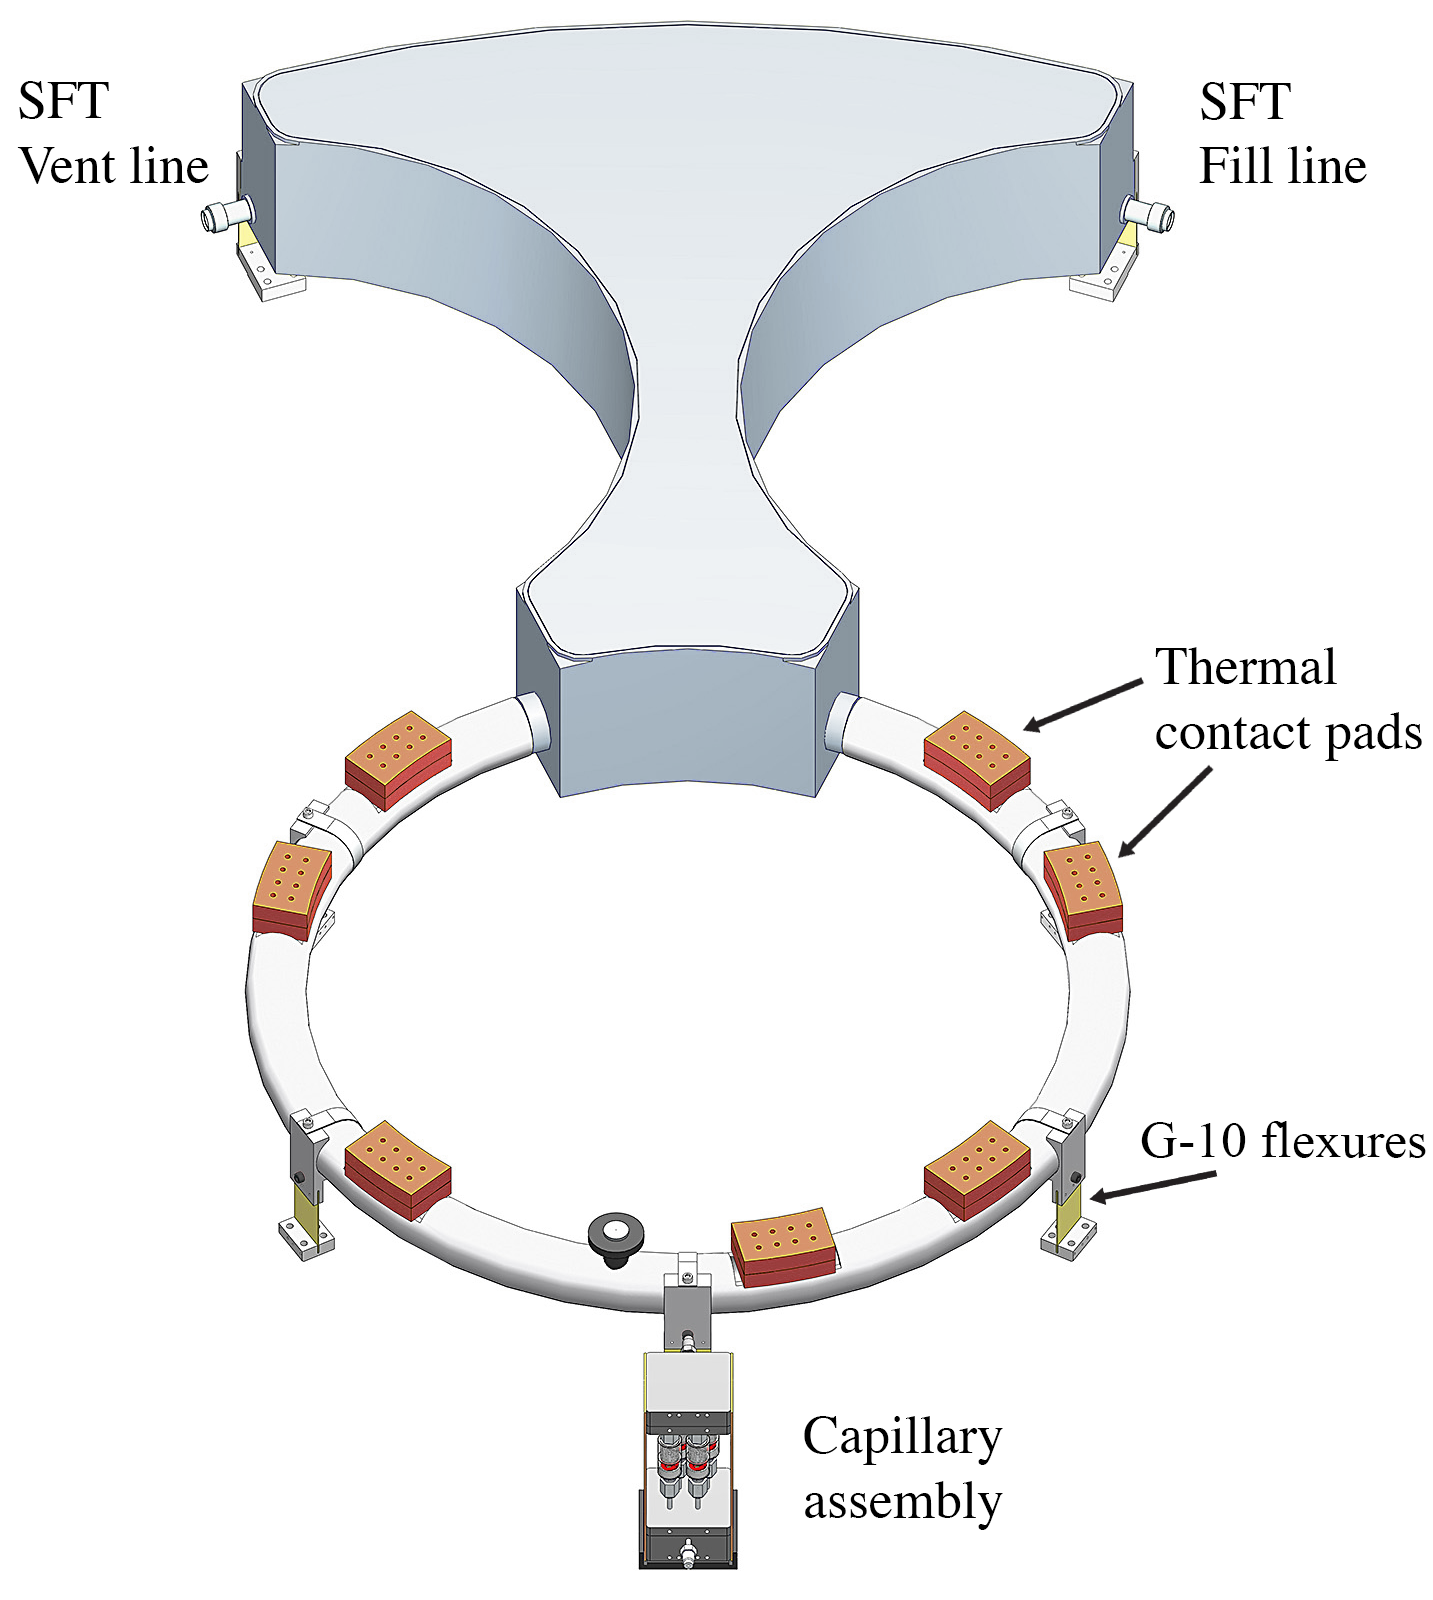
\includegraphics[width = 0.5\textwidth]{img/sft_capassy5.png}   
\end{center}
\caption[The superfluid tank and capillary assembly]{The superfluid
  tank and capillary assembly are mounted to the bottom of the main
  tank. The capillary assembly is located
  just below the SFT ring and connected to both tanks using flexible
  1/8~inch bellows tubing. Thermal contact pads are welded into a ring
  that sits below the main volume. The auxiliary fill line and the vent line exit at the
  top to the right and left respectively. The net volume of the
  superfluid tank is 16~L.}
\label{fig:sft_cap}
\end{figure} 

A number of publications describe capillary systems. Wrubel et al.\ \cite{Wrubel2011} describe a capillary assembly with four parallel polycarbonate capillaries and a needle valve for controlling the flow impedance. Das et al.\ \cite{Das2012} discuss a helium evaporator that is continuously fed by a fixed impedance line. Their measurements of room temperature flow impedance and corresponding cooling power seem to agree with  the results described in the original capillary paper \cite{Delong1970}. Fujiiyoshi et al.\  \cite{Fujiyoshi1991} describe a similar system with comparable results. It is evident that authors arrive at their preferred flow impedance through trial and error and reliance on empirical measurements, see for example \cite{Talpe1988,Singsaas1984}.

Some of the more theoretical aspects of helium superfluidity in capillaries are examined in a paper by Koh \cite{Koh2008}. A simple model that describes the evaporation rate and film creep in a sorption refrigerator is discussed in Lau et al. \cite{Lau2006}. The model helps guide the design parameters of an orifice that prevents undesirable superfluid creep. A large body of literature has investigated the use of capillaries, which are sometimes called \enquote{fixed impedance lines,} in cryogenic applications.

\section{Design}

\subsection{Requirements}
The steady state loading on the superfluid volume shown in Figure
\ref{fig:sft_cap} has been measured during flight-like
conditions. This measurement, made with the superfluid volume empty
and disconnected from the capillary assembly, suggested a steady state
loading of 40~mW. This measurement is consistent with the measured
hold time of the superfluid tank before the capillaries were
installed. Implementing a 1.5~safety factor we conclude that the
capillary assembly must provide at least 60~mW of continuous cooling
power to the superfluid tank.

The superfluid bath must reach a base temperature of at least 1.8~K. This facilitates effective operations of the \hee closed-cycle absorption refrigerators inside each of the six \spider telescopes. Cycling the adsorption refrigerators creates an approximate 5~mW transient loading on the superfluid tank which lasts for an hour. The superfluid tank will have to sustain transients from cycling six refrigerators once every 24-72 hours.

\subsection{Concept}

The \spider capillary system employes three 35~cm long capillaries wrapped around Teflon spools and silver soldered into 1/8~inch \textit{Swagelok} glands with gender preserving VCR fittings (see Figures \ref{fig:cap} and \ref{fig:cap_cross}).\footnote{\textit{Swagelok}, Solon, OH.} Note that Figure \ref{fig:cap} shows an assembly that is able to support four capillaries; the fourth capillary was removed and replaced with caps to reduce loading of the main tank. Having 3--4 capillaries reduces susceptibility to constrictions from potential ice slush in the main tank. Failure of one capillary, most likely due to an ice plug, should not reduce the performance of the superfluid tank if safety factors are chosen appropriately. The capillaries couple two $\sim$50~mL volumes that are connected to the main tank and the superfluid tank through 1/8~inch bellows tubing. The capillary material is extruded SS 304 with a 0.0035~inch inner diameter and a 0.0025~inch wall thickness.\footnote{Capillaries provided by \textit{Eagle Stainless}, Warminster, PA.} The dimensions were chosen to resemble one of the assemblies described in \cite{Delong1970}. 

The net cooling power provided by the system can be changed by simply altering the length of the capillaries that are wound around the teflon spools. This length modification can be obtained without making other changes to the design.  This allows us to quickly arrive at an optimal cooling power by having a collection of interchangeable capsules.

\subsection{Assembly details}

Small, custom-made, brass pucks with 0.009~inch diameter
center-drilled holes are made to fit snugly into the Swagelok
glands. A capillary is threaded through one of the pucks before solder
is allowed to flow into gaps that exist between the gland, puck,
and capillary. The capillaries are then wrapped around hollow Teflon
spools and subsequently routed back into the center of the spools and
through stainless steel compression springs that provide structural
support to the whole assembly while keeping heat conduction at a
minimum. As the capillaries are internal to the springs, there is
little chance that spring compression can pinch the capillaries. The
springs allow us to gently modify the overall length of the assembly
to fit perfectly between the two glands that are welded to each of the
small boxes while conducting negligible heat between the two
temperature stages. Transparent heat-shrink tubing helps align the
Teflon components with the two ends of the VCR fittings and provides
structural rigidity. Together, the capillaries along with VCR
fittings, Teflon components, and springs, are referred to as
capsules. Figure~\ref{fig:cap_cross} shows a cross section of an
individual capsule. %With all components in hand, a trained worker can assemble up to eight functioning capsules in one day.

Stainless steel Mott filters are spot welded to the inside of the
MT~box so as to intercept large particles before they enter the
capillaries.\footnote{Filters purchased from \textit{Mott Corporation}, 
Farmington, CT. We use media grade 20 filters.}  
If correctly installed, the
particle capture efficiency of these filters is such that they collect
99.9\% of particles whose diameter is larger than 20\% of the
capillary diameter. This should allow for effective operations of the
capillaries without contributing significantly to the overall flow
impedance of the system.

\begin{figure}[t]
\begin{center}
\begin{tabular}{c}
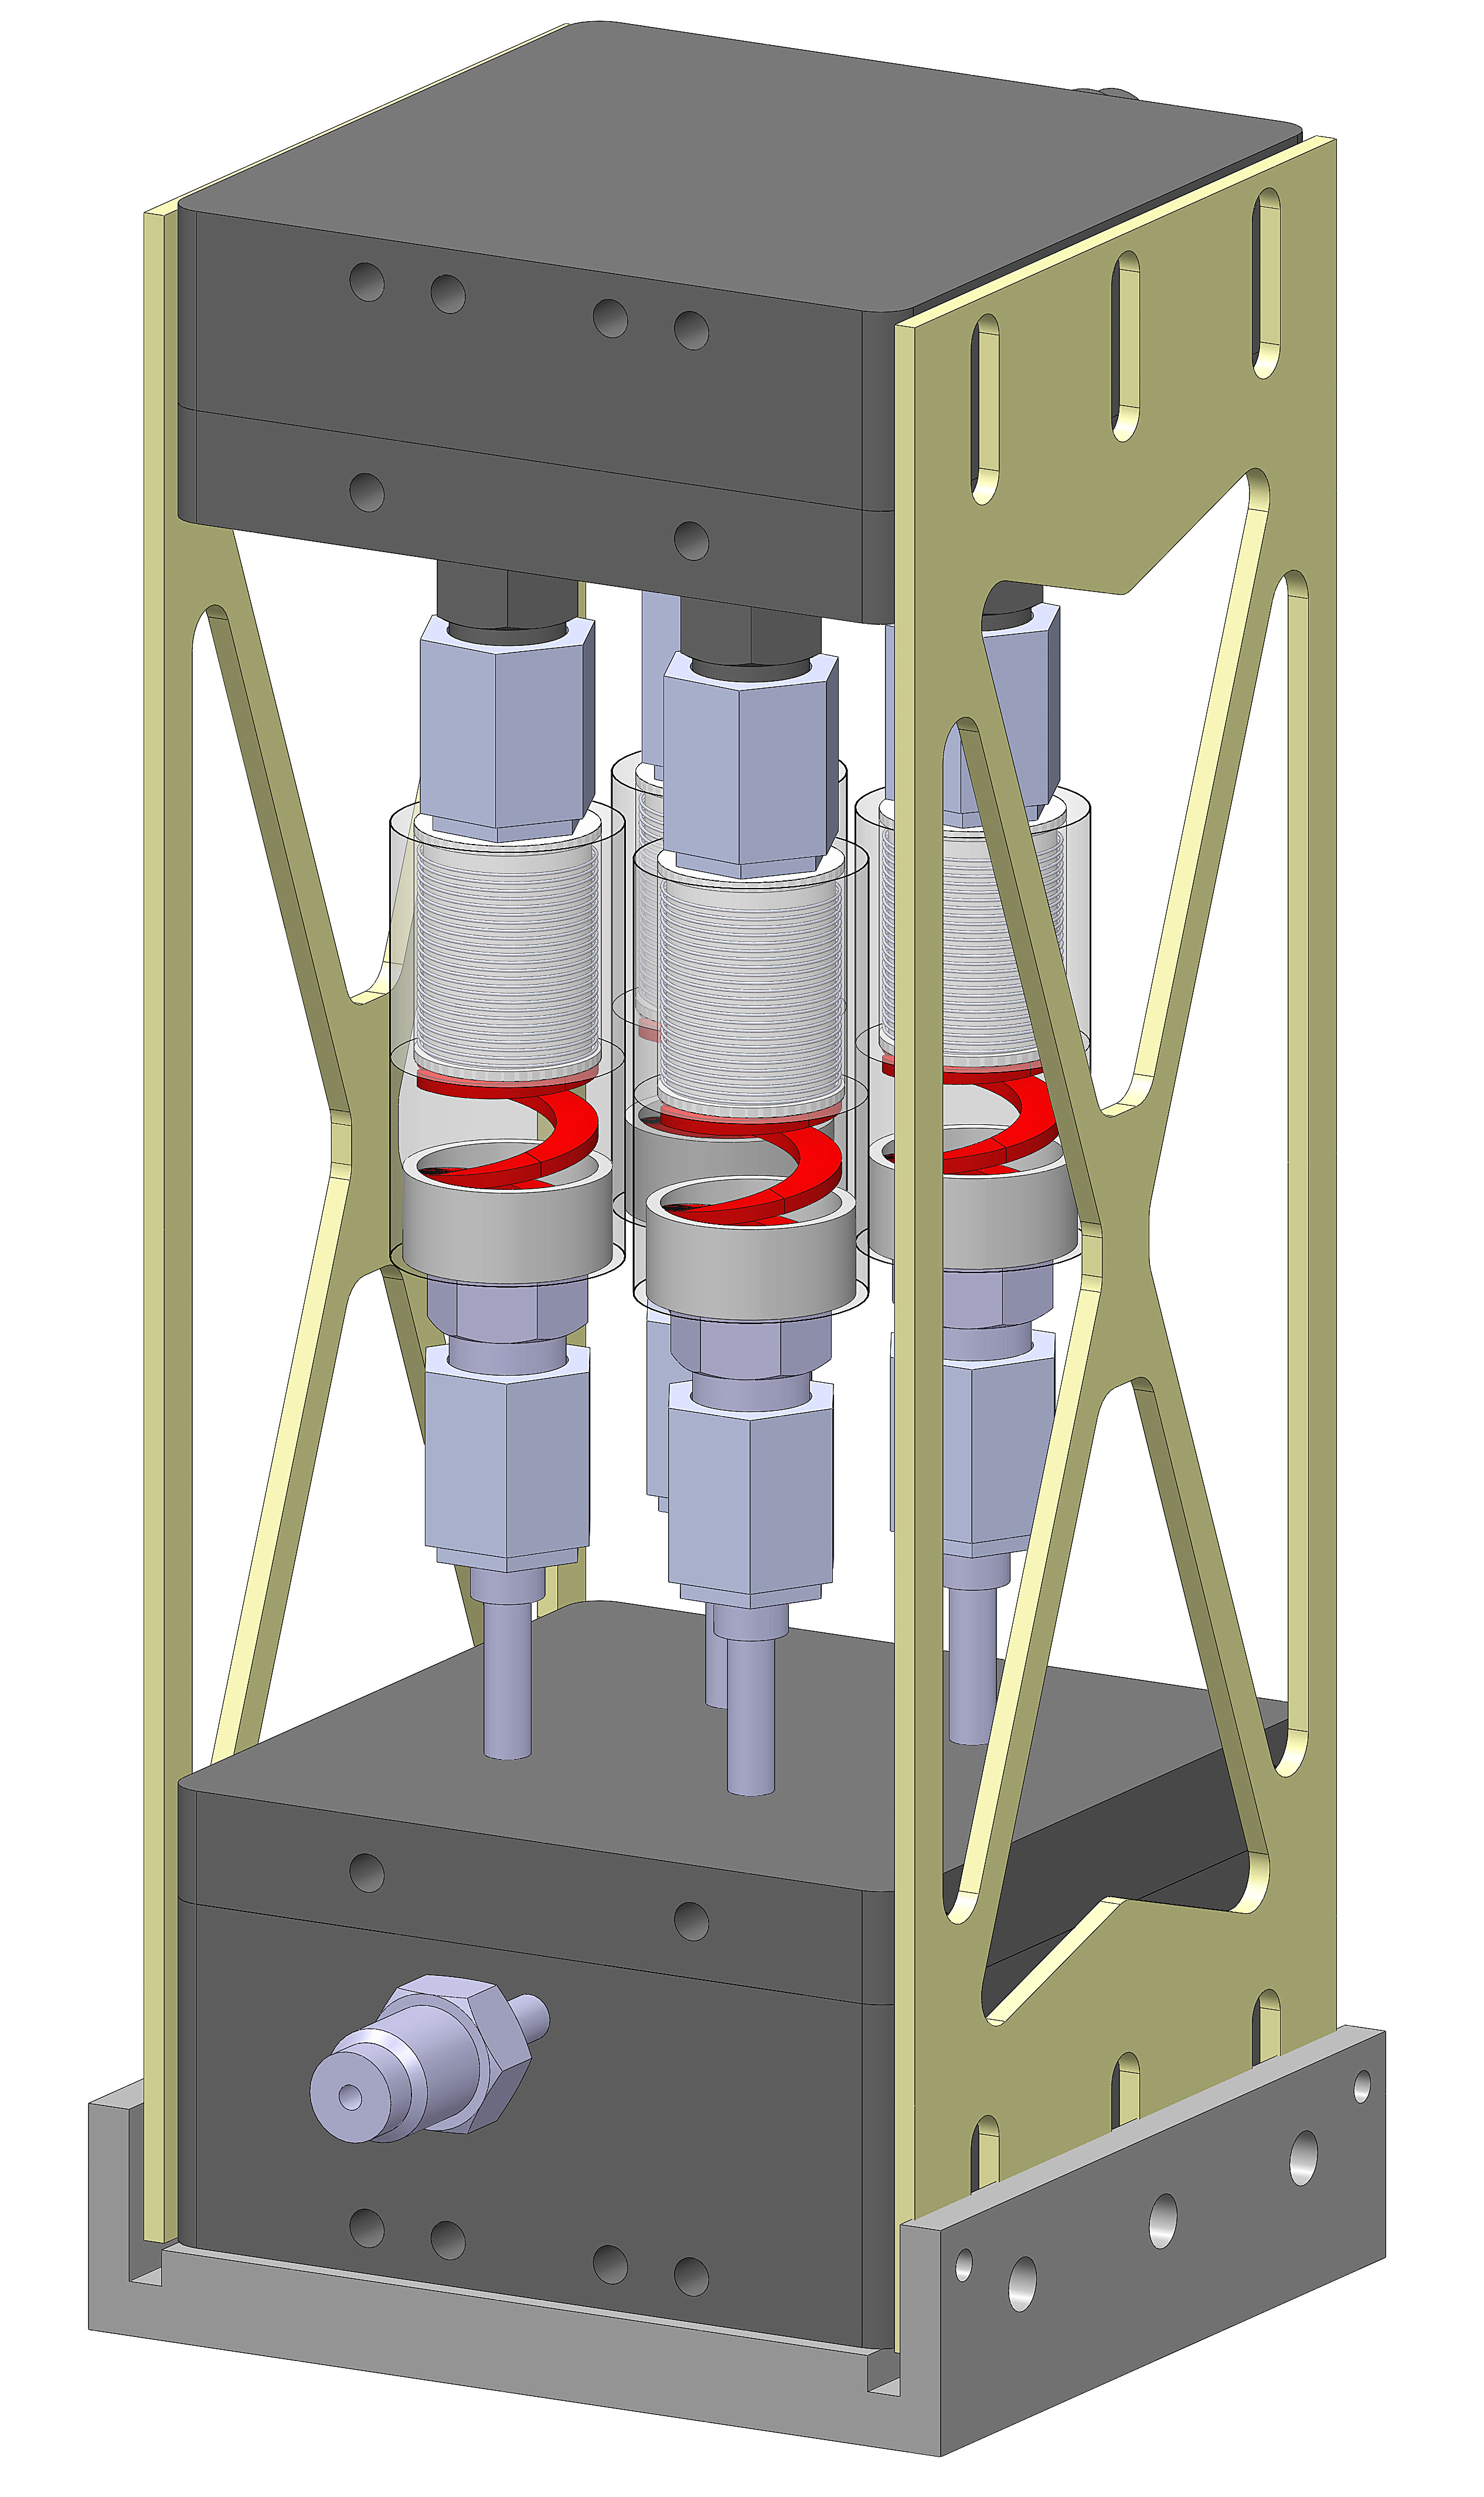
\includegraphics[width = 0.35\textwidth]{img/capassy_vertical3.jpg}
\end{tabular}
\end{center}
\caption[example]
{ \label{fig:cap} The capillary assembly. Four capillaries connect the 4.2~K main tank box (bottom) to the 1.8~K superfluid box (top). The double volume structure is supported by two 1/32" thick G-10 flexures. The thermal load conducted through these flexures is negligible compared to the cooling power from the superfluid. Stainless steel Mott filters located below each capillary prevent ice and other dirt from entering and clogging these high impedance tubing.}
\end{figure}

\begin{figure}[tb]
\begin{center}
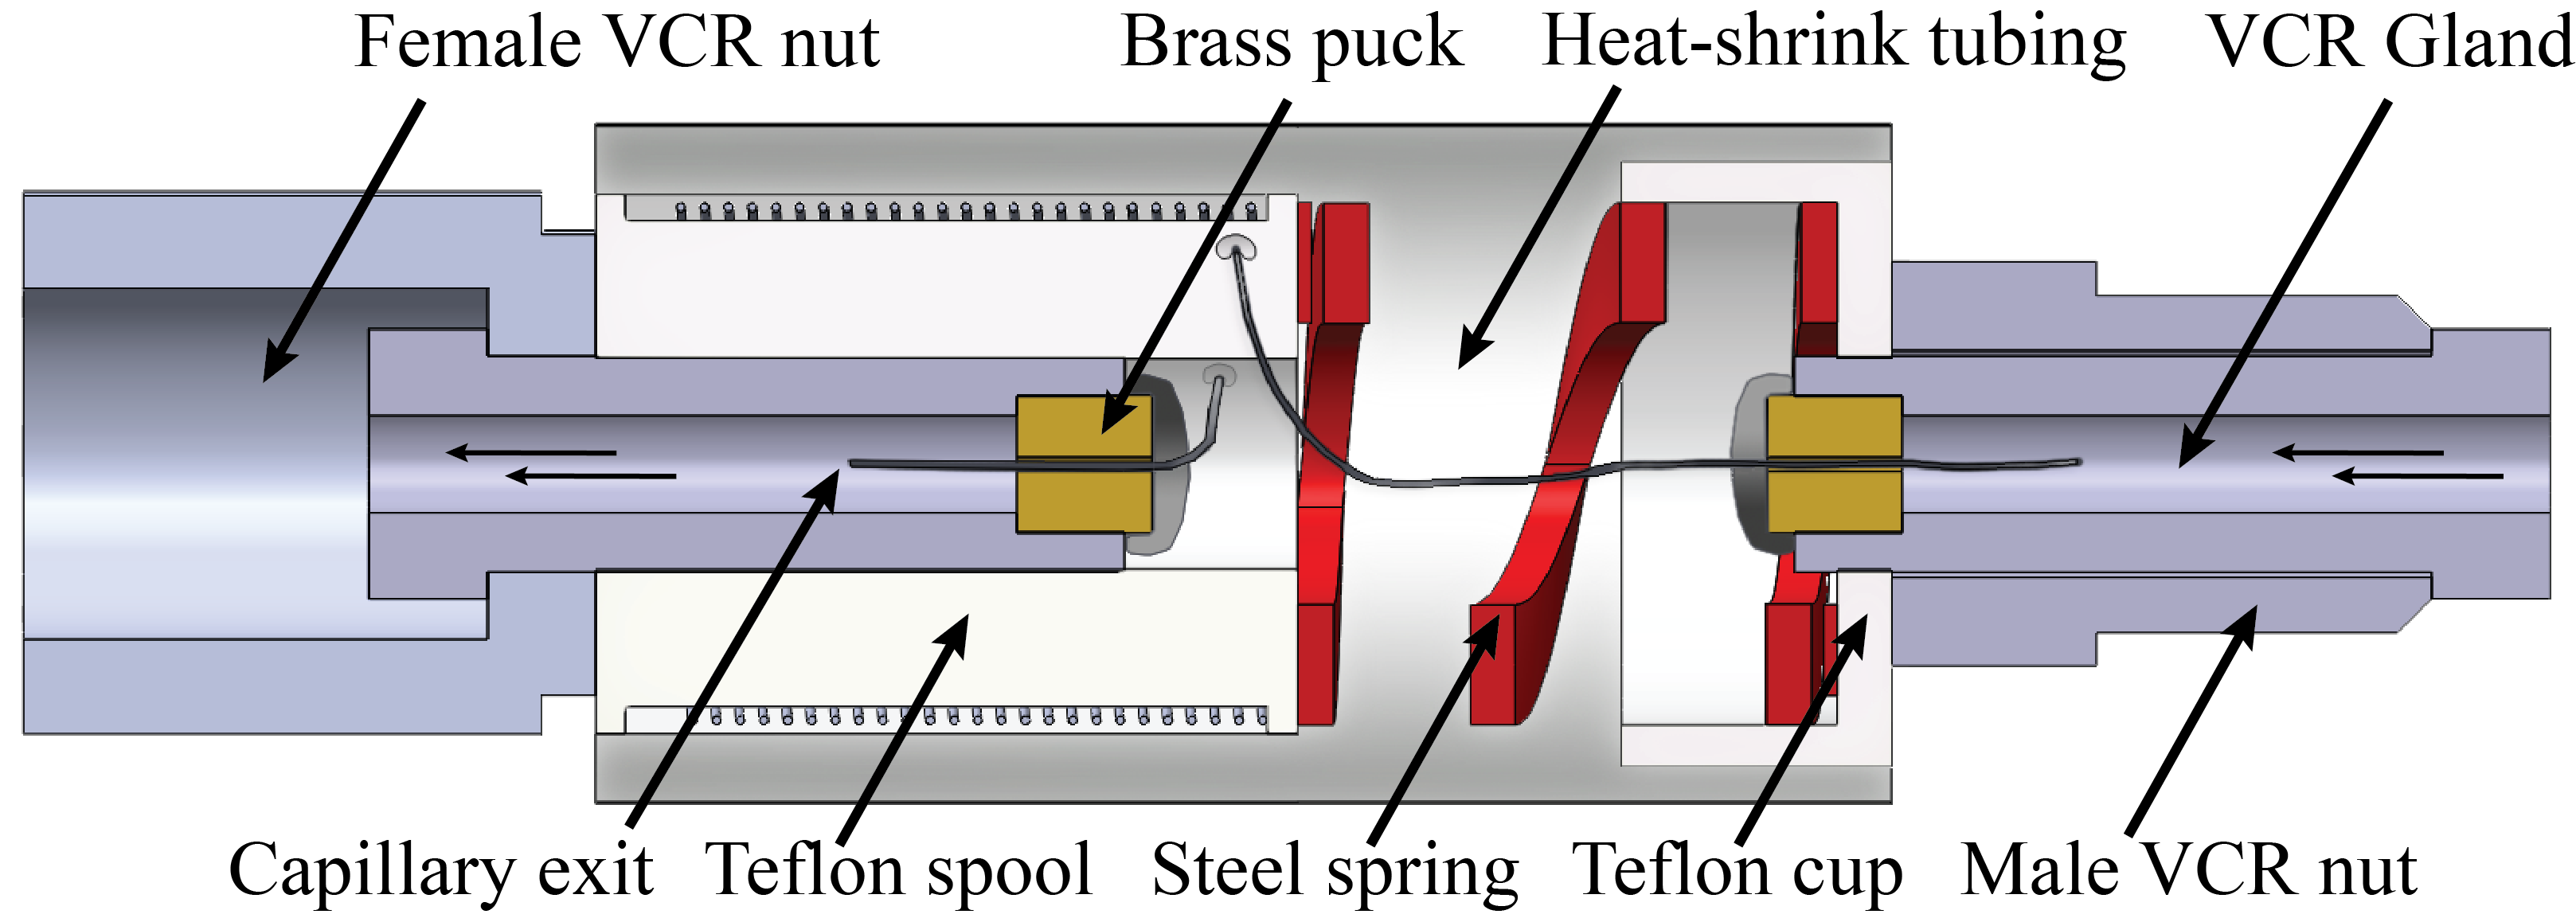
\includegraphics[width = 0.7\textwidth]{img/capillary_cross7.png}
\end{center}
\caption[A cross section through a capsule]{A cross section
  through one of the capsules, measuring 26.3~mm end-to-end. 
  The ends of the capillaries are located
  inside the Swagelok VCR glands, approximately 1~cm from the brass
  pucks. This way, the ends are shielded from mistreatment. After
  having silver soldered the capillary into the puck on the left, the
  capillary is threaded through a small cavity at the edge of the Teflon
  spool. The spool then slides over the gland, after which the
  capillaries are wrapped around the spool. With only a couple of
  inches remaining, the capillary is threaded through another hole at
  the edge of the spool, then through the Teflon cup, after which the
  other end is silver soldered into the brass puck on the right. The
  stainless steel spring is then carefully wrapped around the
  capillary and secured in the Teflon cup. Finally, heat-shrink tubing
  is positioned around both the Teflon components and spring to shield
  the capillaries and unify the assembly. The silver solder is represented
  in this figure by grey pea-shaped objects next to the brass pucks. 
  The direction of helium flow is indicated by small black arrows 
  located inside the VCR glands. 
  }
\label{fig:cap_cross}
\end{figure}


\section{Measuring Capillary Performance}
\label{sec:fund}

Capillary systems are commonly quantified by their cooling capacity, or critical power, $Q_\mrm{crit}$, which is related to the flow rate through the capillaries. The critical power can be estimated through the capillary impedance factor, $Z$, an extrinsic quantity that can be measured at room temperature \cite{Delong1970}. A pressure differential, $\Delta P$, is set up between the two ends of a capillary system and the flow rate measured.\footnote{For example, by watching the pressure increase in a calibrated volume.} The impedance factor is then
\begin{equation}
Z = (1/\eta)\Delta P / \dot{V},
\label{eq:Z}
\end{equation}
where $\eta$ is the dynamic viscosity of the fluid and $\dot{V}$ is the volumetric flow rate. The warm flow impedance can then be compared to the cooling power of the capillaries measured at operational temperatures. 

For the \spider capillary assembly, we measure the flow impedance either on the lab bench or inside the flight cryostat. The latter measurement is performed by pressurizing the main tank to $\sim$15.7~psia, using either nitrogen or helium gas. We then evacuate the superfluid tank and observe the pressure rise in the calibrated volume over hour timescales. The room temperature dynamic viscosity of helium, $\eta (\mrm{He}) = 20.0 \:\mrm{kg/m/s}$, is larger than that of nitrogen, $\eta (\mrm{N_{2}}) = 18.6 \:\mrm{kg/m/s}$ and we account for this in our calculation of flow impedance. It is useful to note that dynamic viscosity is generally proportional to $\sqrt{T}$ \cite{Amdur1947}.

The critical power is measured by applying heat to an empty volume with a steady supply of superfluid helium. The base temperature of the superfluid bath increases with heat input until the superfluid flow is unable to compensate. A temperature runaway effect is then observed where additional heat lifts the temperature of the superfluid enclosure past the \lp at a fast rate. The critical power can also be estimated from the equilibrium flow rate out of the superfluid tank. 

With these measurements in hand, the measured critical power can be compared to the warm flow impedance to establish an empirical relation between the two parameters.

\subsection{Cooling power as a function of warm flow impedance}
\label{sec:hp}

It is difficult to estimate how superfluid helium flow rates depend on the geometry of the capsules. Ideally, the Hagen-Poiseuille equation relates the pressure drop to the length and the diameter of the capillaries as follows
\begin{equation}
\Delta P = \frac{128\eta L\dot{V}}{\pi d^4},
\end{equation}
where $\Delta P$ is the pressure drop over the cylindrical tube with diameter $d$ and length $L$ such that $L \gg d$. Complications arise since the superfluid transition happens somewhere within the capillaries. In the two-fluid model, the above equation is still valid for the normal component whose flow should remain laminar. However, the superfluid component is likely to become turbulent. In this case, the appropriate expression for the heat flow is derived by Schotte \cite{Schotte1984}. The two-fluid model in relation to capillaries is discussed further in Lages et al. \cite{Lages1995}.

\section{Operations in SPIDER}

Two distinct capillary assemblies have been run in the \spider flight cryostat. The current design was installed prior to Run 10 (see Figures \ref{fig:cap} and \ref{fig:cap_cross}). The size and complicated geometry of the superfluid tank, chosen to accommodate six telescopes, heat straps, and the capillaries themselves makes thermal modeling difficult. The following subsection only provides a qualitative description of the thermal system.

\subsection{Thermal architecture}
Both conduction and radiation contribute significantly to the total thermal budget of the superfluid tank. Heat is conducted through the stainless steel vent and fill lines and the G-10 flexures that suspend the superfluid tank from the main tank. Radiation from the inner vapor cooled stage and any light leaks from warmer stages also contribute to the loading at a significant level. Under equilibrium conditions, the enthalpy of the system is kept in balance by the evaporation of liquid helium. We can write the steady-state requirement as follows
\begin{equation}
\dot{m} H_\mrm{vap}(T_\mrm{SFT}) \approx \sum _{\mrm{i}}\int _{T_\mrm{SFT}}^{T = 4 K}  C_\mrm{i} (T')\mrm{d}T' + \sigma _\mrm{SB} A_\mrm{eff}T_{VCS1}^4,
\label{eq:mdot}
\end{equation}
where $\dot{m}$ is the mass flow rate out of the superfluid tank, $H_\mrm{vap}$ is the temperature-dependent enthalpy required to vaporize a unit mass of \hen, $C_\mrm{i}$ represents the conduction through one of the stainless steel or G-10 thermal paths, and the second term on the right-hand-side represents the radiative loading to the SFT, with $A_\mrm{eff}$ corresponding to the effective area of the SFT-VCS1 system. From this we see that the equilibrium temperature of the SFT depends on the flow rate. As the vapor pressure of the of helium bath is set by the pumping capacity and the impedance of the capillaries, so will the equilibrium temperature of the liquid bath.

If the impedance of the capillaries is sufficiently low, the flow from the main tank will negate any liquid loss and an equilibrium state should be reached. The equilibrium temperature of the liquid bath, $T_\mrm{eq}$, should to first order only depend on the pumping rate of the pump and the impedance of the capillaries. The temperature of the superfluid volume as measured by thermometer located on the outside of the aluminum tank will however also depend in a complicated way on the geometry of the tank and its location relative to thermal links. %No attempts have been made at predicting the equilibrium temperature of the system.

Measurements show that the capillary assembly provides approximately
100~mW of cooling power to the superfluid volume while conducting only
2~mW between the two temperature stages. This corresponds to an
equilibrium flow through the capillaries of about $2.0\pm0.5$~SLPM.\footnote{
SLPM stands for Standard Liter Per Minute, where standard refers to 
273.15~K temperature and 1~atm pressure. For \hen, we find that 2.00 SLPM corresponds to 5.87~mg/s.} 
By boiling off the SFT and measuring the flow rate we estimate an
equilibrium superfluid liquid volume of approximately 2.0~L, only 1/8~of the
total volume of the SFT. This value is mainly determined by the
geometry and capillary flow rates.

\subsection{Cryogenic operations}

%The large size of the cryogenic system makes full cool down quite slow. It is also well known that capillaries tend to plug.

The capillaries are at risk of becoming plugged, most likely with nitrogen ice, in the interim between liquid nitrogen pre-cooldown and the initial liquid helium fill. The process is inherently risky as residual nitrogen can solidify in the presence of liquid helium; it is fair to assume that full risk mitigation is impossible without moving parts. So far, we have not devised an operating procedure with a 100\% success rate.

Given the long response time of the large cryostat, and the tight schedule afforded by McMurdo ballooning, flow constriction in the capillaries poses significant risk to the schedule. In the worst case scenario, plugged capillaries could require heating the cryostat back up to room temperature and breaking vacuum, causing a 2--3 week slip in schedule at minimum. So far, however, we have been successful in clearing plugged capillaries by suspending liquid helium cool downs and heating the capillaries (which are well isolated from the main tank) up to 300~K. This procedure requires approximately 2-3 days, and so far, it has a 100\% success rate. 

The initial cool-down stage involves filling the main tank with few hundred liters of liquid nitrogen while pressurizing the superfluid tank to 6~psig with gaseous helium and maintaining approximately 1~SLPM of flow out of a pressure regulator on the SFT vent. Once all liquid nitrogen has boiled out, the main tank is evacuated. The system is then backfilled with gaseous helium at room temperature. We maintain the capillary assembly at room temperature during the initial cool-down phase, approximately 270~K rather than 90~K. This should ward off  flow restrictions. This has to be done carefully, however, as overheating might damage the capillaries.

Immediately following helium backfilling of the main tank we perform a capillary flow test to determine the status of the capillaries before initial liquid helium transfer. The flow test is performed with an approximately 90~K main tank pressurized to 15--16~psia with gaseous helium. The superfluid tank is then evacuated with a scroll pump attached to the SFT vent line manifold which is connected to an absolute pressure gauge. After evacuation, we valve off the scroll pump and observe pressure rise in the 16--18~L volume of the superfluid tank and manifold. The pressure increase is due to flow through the capillaries, driven by the roughly 16~psi pressure differential. The rate of pressure increase as measured on the manifold depends in a non-trivial way on temperature of the main tank, capillaries, superfluid tank, and the room. As these sub-systems can have different temperatures at the time that the flow test is performed, we have to correct for this in estimating the performance of the capillaries. 

%This paper estimates the critical power of a few capillary systems. The authors estimate that a 2.25~m cupronickel capillary with a 0.1~mm ID provides a critical power of 15~mW to a superfluid volume. We base our capillary design on this particular capillary. Implementing four capillaries should then provide a critical power of about 60~mW which roughly corresponds to an upper bound on the loading to the SFT. Here, critical power is the amount of power that needs to be applied to a superfluid volume in order to see a temperature increase from the superfluid base temperature.

%The system that's currently under testing is a 316 SS capillary that is 1.52~m long, an ID of 0.09~mm, and a 0.20~mm OD.

%The authors define a quantity $Z$, called the impedance factor, to be calculated from measurements of the capillary system at room temperature. A pressure differential, $\Delta P$, is set up between the two ends of the capillary system and the flow rate measured. The impedance factor is then
%\begin{equation}
%Z = (1/\eta)\Delta P / \dot{V},
%\end{equation}
%where $\eta$ is the viscosity of the fluid and $\dot{V}$ is the volume flow rate. The cupronickel capillary is measured to have $Z = 0.67 \times 10^{-12} \:\mrm{cm^{-3}}$.

%\red{Our measurement of warm flow impedance does not appear to scale to cooling power in the same way as DeLong et al. Using DeLong's empirical scaling law we will overestimate the cooling capacity of the capillaries. We need to describe this problem in an elegant way.}

%Capillaries are not superleaks, geometrical shapes impermeable to normal-fluid, rather, they should be though of as physical connections with very high flow impedance.

%We've measured the warm flow rate in the SPIDER capillary system and found it to be $0.026\:\mrm{cm^3/s}$ through the four capillaries. This corresponds to a single capillary impedance factor of about $Z_\mrm{S} = 0.11 \times 10^{-12} \:\mrm{cm^{-3}}$. Table \ref{tab:flowrates} shows typical values obtained from flow test at various temperatures. A comparison with these measurements to that of DeLong suggest that the capillary system will provide more than 60~mW of cooling power to the SFT.

%\begin{table}[]
%\caption{Results of helium flow tests at various temperatures. The table shows the values for the driving pressure, the temperature of the capillaries, the flow rate, and the He viscosity. The 4~K measurement is not performed with the system in a steady state. \label{tab:flowrates}}
%\begin{center}
%\begin{tabular}{llll} \hline
%\rule[-1ex]{0pt}{3.5ex}  \textbf{$\Delta P$} &  \textbf{$T$} & \textbf{$\dot{m}$} & \textbf{$\eta$} \\
%\hline
%\rule[-1ex]{0pt}{3.5ex} $22 \:\mrm{psi}$ & $300 \:\mrm{K}$ & $8.9 \times 10^{-4} \frac{\mrm{mole}}{\mrm{s}}$ & $200 \:\mrm{\mu P}$ \\
%\hline
%\rule[-1ex]{0pt}{3.5ex} $22 \:\mrm{psi}$ & $77 \:\mrm{K}$ & $2.2 \times 10^{-3} \frac{\mrm{mole}}{\mrm{s}}$ & $80 \:\mrm{\mu P}$ \\
%\hline
%\rule[-1ex]{0pt}{3.5ex} $22 \:\mrm{psi}$ & $\approx 4 \:\mrm{K}$ & $4.3 \times 10^{-2} \frac{\mrm{mole}}{\mrm{s}}$ & $28 \:\mrm{\mu P}$ \\
%\hline
%\end{tabular}
%\end{center}
%\end{table}

%A number of flow measurements were performed as the system was at 4~K. Unfortunately, none of those measurements were performed with the system in a steady state. An IONIVAC ITR90 ionization gauge was used to read the pressure increase as a small calibrated volume filled with helium. We expect that high non-equilibrium flow rates result in an overestimate for flow rate through the capillaries at these temperatures. We note, however, that even the 77~K flow measurement suggests a cooling power of about 100~mW.

%\subsection{Theory}
%Superfluid is a by characterized by inviscid flow of zero entropy liquid with almost infinite thermal conductivity. It is is observed when liquid helium-4 is cooled below a 2.17~K referred to as the $\lambda$-point. This phenomenum was first discovered in 1937 by Kapitsa, Allen, and Misener, and later garnered a phenomelogical description for which Landau received the Nobel prize in 1962. In this section we will briefly review the theory of superfluidity in relation to capillaries.

%The elegant theory of superfluidity is contrasted by a medley of empirical evidence.
 
\section{Experimental Results}
% The superfluid tank and capillaries are shown in Figures \ref{fig:cap} and \ref{fig:sft_cap}. Superfluid helium exits the capillaries in the smaller of the two boxes which is connected to the superfluid tank through 6" long bellows tubing with a 1/8" diameter.

%The equilibrium temperature of the liquid bath, $T_\mrm{eq}$, should to first order only depend on the pumping rate of the pump and the impedance of the capillaries. The temperature of the superfluid volume as measured by thermometer located on the outside of the aluminum tank will however also depend in a complicated way on the geometry of the tank and its location relative to thermal links. No attempts have been made at predicting the equilibrium temperature of the system.

\subsection{Performance history}

Table~\ref{tab:capprop} shows the measured properties of the capillary assemblies for the cryogenic runs where we have a definitive measurement of the flow rate through the capillaries. 

During Run 9 (the first run with the capillaries in the cryostat) we found that the cooling power of the capillaries was not sufficient to sustain a reasonable amount of superfluid. This was surprising, as we expected approximately 40~mW of cooling power based on the warm flow impedance measurement and the results of DeLong et al.\ \cite{Delong1970}. Prior to Run 10, we chose to increase the throughput of the capillaries assuming that the critical power would greatly exceed the heat input to the superfluid system. At that point we found that the pumping rate of our dry scroll pump was limiting the minimum temperature of the system (see Eq.~\ref{eq:mdot}). Another pump was acquired before run 11 and one of the capsule was removed to reduce the capillary throughput and therefore the loading to the main tank. Run 11 performance was ideal.

Some flow restriction appear to have formed during Run 12, as we observed greatly reduced throughput given expectations from the warm flow impedance. Even at decreased flow rate, we were still able to efficiently cool both telescopes installed for that run. Run 14 (as well as subsequent runs) shows a non-negligible increase in the warm flow impedance compared to previous runs. It is possible that one of the three capillaries has been damaged in a way that permanently restricts flow.

%The warm flow impedance measured prior to Runs 14 and 15 are significantly different from Runs 11--13. It is possible that one of the three capillaries has been damaged in a way which permanently restricts flow.

We note that warm flow impedance is generally a great predictor for superfluid flow. This is clear from the consistency of the product $ Z \times f_\mrm{SFT}$, shown in the last row of Table~\ref{tab:capprop}.

\begin{table*}[]
\caption[Measured properties of various capillary assemblies]{Measured properties of various capillary assemblies. Warm flow impedance was measured using flow tests at 300\,K. Critical power was measured by applying heat to the superfluid volume and observing the power at which the capillaries couldn't provide sufficient cooling power. Finally, equilibrium flow rate was measured by attaching a flow meter to the exhaust line of the pump that was pumping on the superfluid tank. Note that in our measurements, the product of warm flow impedance and flow rate out the SFT is roughly constant, with one exception.
}%For Run 9 the cooling power of the capillaries was less than the total equilibrium heat input to the superfluid tank. The throughput of the capillaries was greatly increased between Runs 9 and 10 such that the pumping speed limited the equilibrium temperature of the superfluid tank. A flow restriction formed during Run 12, which limited the superfluid flow rate. 
\label{tab:capprop}
\begin{center}       
\begin{tabular}{@{} l L L L L L L @{} >{\kern\tabcolsep}l @{}} 
\toprule
\textbf{Property} & DeLong & \textbf{R9} & \textbf{R10} & \textbf{R11} & \textbf{R12} & \textbf{R13} & \textbf{R14} \\
\midrule
\begin{minipage}[t]{0.33\columnwidth}Impedance, $ Z \times10^{9} \:[\mrm{cm}^{-3}] $\end{minipage} & $670$ & $240$ & $36$ & $47$ & 41 & 49 & 59  \\
\begin{minipage}[t]{0.33\columnwidth}Critical power, $Q_\mrm{crit}$ [mW] \end{minipage} & 15 & 18 & 154 & N/A & N/A & N/A & N/A \\
\begin{minipage}[t]{0.33\columnwidth}Eq.\ flow, $f_\mrm{SFT}$ [SLPM] \end{minipage} & 0.44 & 0.45 & 3.1 & 2.5 & 0.65 & 2.2 & 1.7 \\
\begin{minipage}[t]{0.33\columnwidth}$Zf_\mrm{SFT}$ [$10^9\,\mrm{SLPM}/\mrm{cm}^{3}$] \end{minipage} & 295 & 109 & 112 & 118 & 27 & 107 & 100  \\
\bottomrule
\end{tabular}
\end{center}
\end{table*} 

\subsection{Relation between warm flow impedance and cooling power}

The warm flow impedance of the capillary system has been measured before every cryogenic run using the method described in Section \ref{sec:fund}. Unfortunately, we do not however have measurements for the superfluid flow rate and/or the 80\,K flow rate for some of the more recent cryogenic runs. This is largely because our flow meter stopped working after run 14 and we failed to conduct reliable 80\,K flow tests prior to Run 11.

Thankfully, cryogenic runs 9--14 provide us with valuable constraints on the relation beteween warm flow impedance and superfluid flow rates. We find that using the relation described in \cite{Delong1970} our measurement of the warm flow impedance overestimates the critical power by a factor of three, but in a repeatable manner (see last row in Table \ref{tab:capprop}). It is possible that the designs differ, for example, with regards to geometry, in some crucial way. DeLong et al.\ \cite{Delong1970} measure flow impedance with a 3.1~torr pressure differential whereas our measurement is performed with roughly 800~torr driving the flow. 

Direct measurements of critical power were only performed for Runs 9 and 10. We know, however, that the results scale linearly with equilibrium superfluid flow. Taken at face value, the load tests conducted during runs 9 and 10 suggest a cooling power of 40 and 50\,mW/SLPM, respectively. We note that \cite{Delong1970} observed a roughly 50\% cooling efficiency, corresponding to about 34\,mW/SLPM (see discussion in Section \ref{sec:lit}).

Figure \ref{fig:flowvsz} shows the relation between warm flow impedance, $Z$, and the equilibrium flow rate out of the superfluid tank, $f_\mrm{SFT}$. The best fit linear relation to all points, except the outlier from run 12, suggests 
\begin{equation}
f_\mrm{SFT} = (-0.0616 \cdot 10^{9} \times Z + 5.315) \quad [\mrm{SLPM}].
\end{equation}
The corresponding cooling power can be obtained from the flow rate by multiplying by with 34\,mW/SLPM. In other words, 1\,SLPM is expected to provide about 34\,mW of cooling power to the superfluid stage. Note that we quote SLPM at 273\,K and that the density of helium at $0^{\circ}$\,C corresponds to roughly 0.176\,g/L. Also note that we only expect this approximate linear relationship to hold in the narrow region of flow impedances we are probing here.

Finally, we note that an experimental effort that accurately maps cold flow rates as a function of warm flow impedances over a significant range of impedance values would be worthy of publication. Surprisingly, such results are essentially missing from the literature.

\begin{figure*}[t]
\begin{center}
\makebox[\textwidth][c]{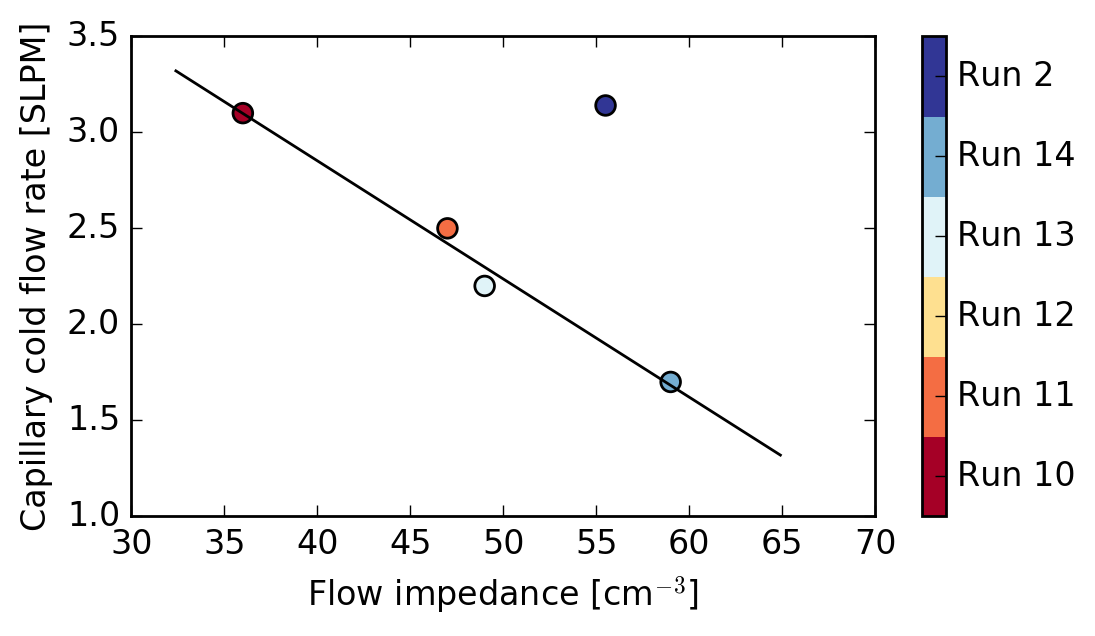
\includegraphics[width = 0.80\textwidth]{img/impedance_vs_cold.png}}
\end{center}
\caption[Cold flow rate vs warm flow impedance]{Cold flow rate, $f_\mrm{SFT}$, as a function of warm flow impedance, $Z$. We observe a clear linear relation between the results from Runs 10, 11, 13, and 14.}
\label{fig:flowvsz}
\end{figure*} 

\subsection{Quality factor}
\label{sec:qf}

The relation between warm flow impedance and superfluid flow presented above can be useful. However, we need to be able to gauge capillary health with the flight cryostat parked at 80\,K just before we intend to fill the main tank with helium. Here, things get a bit more complicated because the temperature profile of the capillaries, and therefore the temperature of the main tank and the superfluid tank have a non-negligible effect on the outcome of any flow test. Of course, our flow tests are performed by measuring pressure rise in a 300\,K volume that is isobaric to another volume wherein gas resides at a much lower temperature. All of this information should somehow be factored into physically motivated estimator that correlates with measured superfluid flow rates.

Unfortunately, we have limited data that we can justify using as a training set for our model. Only data from runs 11, 13, and 14 are suitable for this purpose. Using those data, we derive a dimensionless quality factor, $Q$, that scales linearly with observed superfluid flow. The physically motivated parametrization goes as
\begin{align}
Q &\equiv \frac{\eta (T_\mrm{cap})}{\Delta P} \frac{V_\mrm{SFT}+V_\mrm{man}}{T_\mrm{eff}} \left( \frac{d p}{d t} \right), \\
T_\mrm{eff} &\equiv \frac{\alpha T_\mrm{SFT}+T_\mrm{room}}{1+\alpha},
\end{align}
where $V_\mrm{SFT}$ and $V_\mrm{man}$ represent the volume of the superfluid tank and the outside manifold, respectively, $\Delta P$ is the pressure differential between the main tank and superfluid tank, $\eta$ is the effective dynamic viscosity of the gas traveling through capillaries at temperature $T_\mrm{cap}$, $T_\mrm{SFT}$ is the average temperature of the superfluid tank, $T_\mrm{room}$ is the room temperature, and $(d p/d t)$ is the rate of pressure increase in the superfluid tank during the flow test. Finally, $\alpha$ is a parameter that we use to fit our model to the realized behavior. In our system, we find that setting $\alpha \approx 0.5$ maximizes the correlation between $Q$ and realized flow rates.

Figure \ref{fig:quality_factor} shows the superfluid flow rate as a function of the quality factor as calculated from 80\,K flow tests. On average, the quality factor mirrors the realized flow rates. This relationship should hold for future cooldowns as long as the warm flow impedance of the capillary assembly stays within the range that we have probed so far. The best fit linear relationship is 
\begin{equation}
f_\mrm{SFT} = 0.863 \times Q \quad [\mrm{SLPM}].
\end{equation}
By calculating the quality factor, we can forecast the cooling power of the capillary system and determine whether the cryostat is ready to be filled with liquid helium.\footnote{The initial helium fill is time consuming. The process normally starts in the early morning and is rarely over at a reasonable hour. The ability to quickly ascertain the health of the capillaries is essential.}

Finally, we note that the quality factor for runs 14, 15, 16, and Run 2 in the new flight cryostat was measured to be 1.96, 2.10, 1.92, and 1.66, respectively. This corresponds to a superfluid flow rate of 1.7, 1.8, 1.7, and 1.4\,SLPM, respectively. An equilibrium flow rate of 1.4\,SLPM corresponds to a cooling power of 47\,mW. This doesn't leave much margin for error.

\begin{figure*}[t]
\begin{center}
\makebox[\textwidth][c]{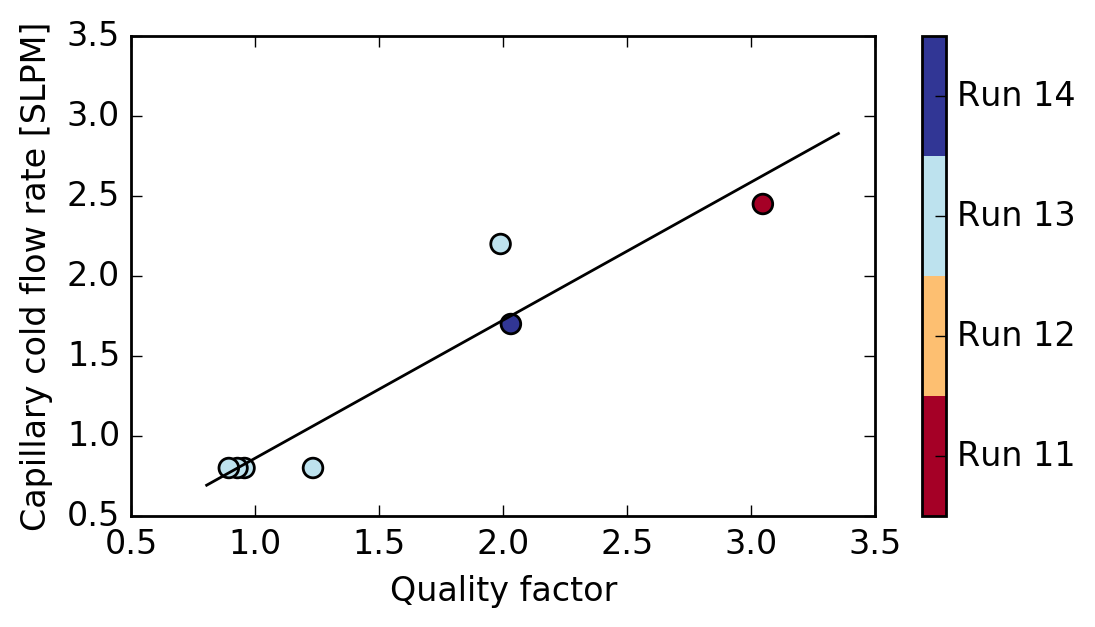
\includegraphics[width = 0.80\textwidth]{img/q_vs_cold.png}}
\end{center}
\caption[Superfluid flow rate as a function of quality factor.]{Superfluid flow rate as a function of quality factor.}
\label{fig:quality_factor}
\end{figure*} 

\subsection{Rough motivation for validity of quality factor}

For a fixed volume and temperature, the ideal gas equation tells us that 
\begin{equation}
\frac{dp}{dt} = \frac{dn}{dT} \left(\frac{RT}{V} \right),
\end{equation}
where $R = 8.31\,\mrm{J/K/mole}$ is the gas constant. Since the molecular flow through the capillaries is filling two isobaric volumes, the SFT and the outside manifold, we know that the pressure in the two volumes is equal, $p_1(t)=p_2(t)$. This also means that for any time $t$
\begin{equation}
\frac{n_1 (t) RT_1}{V_1} = \frac{n_2 (t) RT_2}{V_2}.
\end{equation}
From this we can see that 
\begin{equation}
\frac{d n_1}{dt} = \left( \frac{V_1T_2}{V_2T_1} \right) \frac{dn_2}{dt},
\end{equation}
and therefore
\begin{align}
\frac{d n}{dt} &= \frac{d}{dt}(n_1+n_2) \nonumber \\ 
&= \left( 1 + \frac{V_1T_2}{V_2T_1} \right) \frac{dn_2}{dt} \nonumber \\
&= \left( \frac{V_2}{RT_2} + \frac{V_1}{RT_1} \right) \frac{dp}{dt}
\label{eq:dndt}
\end{align}
where in the last step we simply used the fact that
\begin{equation}
\frac{dn_2}{dt} = \frac{V_2}{RT_2} \frac{dp_2}{dt}.
\end{equation}

The Hagen-Poiseuille equation also tells us that $dn/dt \propto \Delta P /\eta$ if the capillaries and gas are isothermal (see discussion in Section \ref{sec:hp}). If we plug this assumption into Equation \ref{eq:dndt}, we obtain
\begin{equation}
Q \frac{\Delta P}{\eta} = \left(\frac{V_1}{RT_1} + \frac{V_2}{RT_2} \right) \frac{dp}{dt},
\end{equation}
where $Q$ is some constant with strange units. Rearranging, we arrive at the following expression
\begin{equation}
Q = \frac{\eta }{\Delta P} \left( \frac{V_\mrm{SFT}}{RT_\mrm{SFT}}+\frac{V_\mrm{man}}{RT_\mrm{man}} \right) \left( \frac{d p}{d t} \right).
\end{equation}
where we have assigned the indices 1 and 2 to the SFT and manifold, respectively. This expression seems physically motivated, but unfortunately, it doesn't seem to fit our data very well. Instead, we use a slightly different version, namely
\begin{equation}
Q = \frac{\eta }{\Delta P}\frac{V_\mrm{SFT}+V_\mrm{man}}{RT_\mrm{eff}} \left( \frac{d p}{d t} \right),
\label{eq:q}
\end{equation}
with 
\begin{equation}
T_\mrm{eff} \equiv \frac{\alpha T_\mrm{SFT}+T_\mrm{room}}{1+\alpha}.
\end{equation}
We find that a very large value of $\alpha$ tends to yield the best agreement with observations, suggesting that the effective temperature that we should use in the above expression is that of the SFT. 

%, and assumed that there exists a temperature  $T_\mrm{eff}$ such that
%\begin{equation}
%\left( \frac{V_1}{RT_1} + \frac{V_2}{RT_2} \right) \approx \frac{V_1+V_2}{RT_\mrm{eff}},
%\end{equation}
%with 
%\begin{equation}
%T_\mrm{eff} \equiv \frac{\alpha T_\mrm{SFT}+T_\mrm{room}}{1+\alpha}.
%\end{equation}

When comparing flow through two capillary systems with different physical properties, it is clear that a larger value of $Q$ is indicative of lower flow impedance. Equation \ref{eq:q} can therefore be used to obtain a comparison between different realizations of capillary systems. Furthermore, we find that by inputting $\eta$, $\Delta P$, $V$, $T$, $dp/dt$ in units of Poise, psia, L, K, and torr/min, the above equation outputs a number that is close to $10^{-9}$ for the \spider capillary system. Multiplying with $10^9$ and plotting cold flow rates in units of SLPM as a function of $10^{9} \times Q$ as measured during 80\,K flow tests, we not only observe strong correlation between the two parameters, we also find that the two numbers roughly agree (see discussion in Section \ref{sec:qf}). By calculating $Q$ we therefore seem obtain a prediction for the resultant superfluid flow rate in units of SLPM. 

\subsection{Temperature profiles}

%Thermometers along the superfluid tank allow us to monitor the temperature profile of the superfluid tank, and to some extent, gauge the superfluid liquid level inside the tank (see Figure~\ref{fig:sft_hist}). %The equilibrium flow rate is continuously monitored using flow meters calibrated for low flow rates which we install on the exhaust of our scroll pumps.\footnote{\textit{Omega Engineering Inc.}, Stamford, CT.}

Thermometers along the superfluid tank allows us to monitor the temperature profile of the superfluid tank and to some extent gauge the superfluid liquid level inside the tank. Measurements show that the capillary box is at an elevated temperature with respect to the rest of the superfluid assembly even though it is at the lowest gravitational potential. We have also observe periodic temperature oscillations at 10-100~mHz which have hitherto not been given a good explanation.

\begin{figure*}[t]
\begin{center}
\makebox[\textwidth][c]{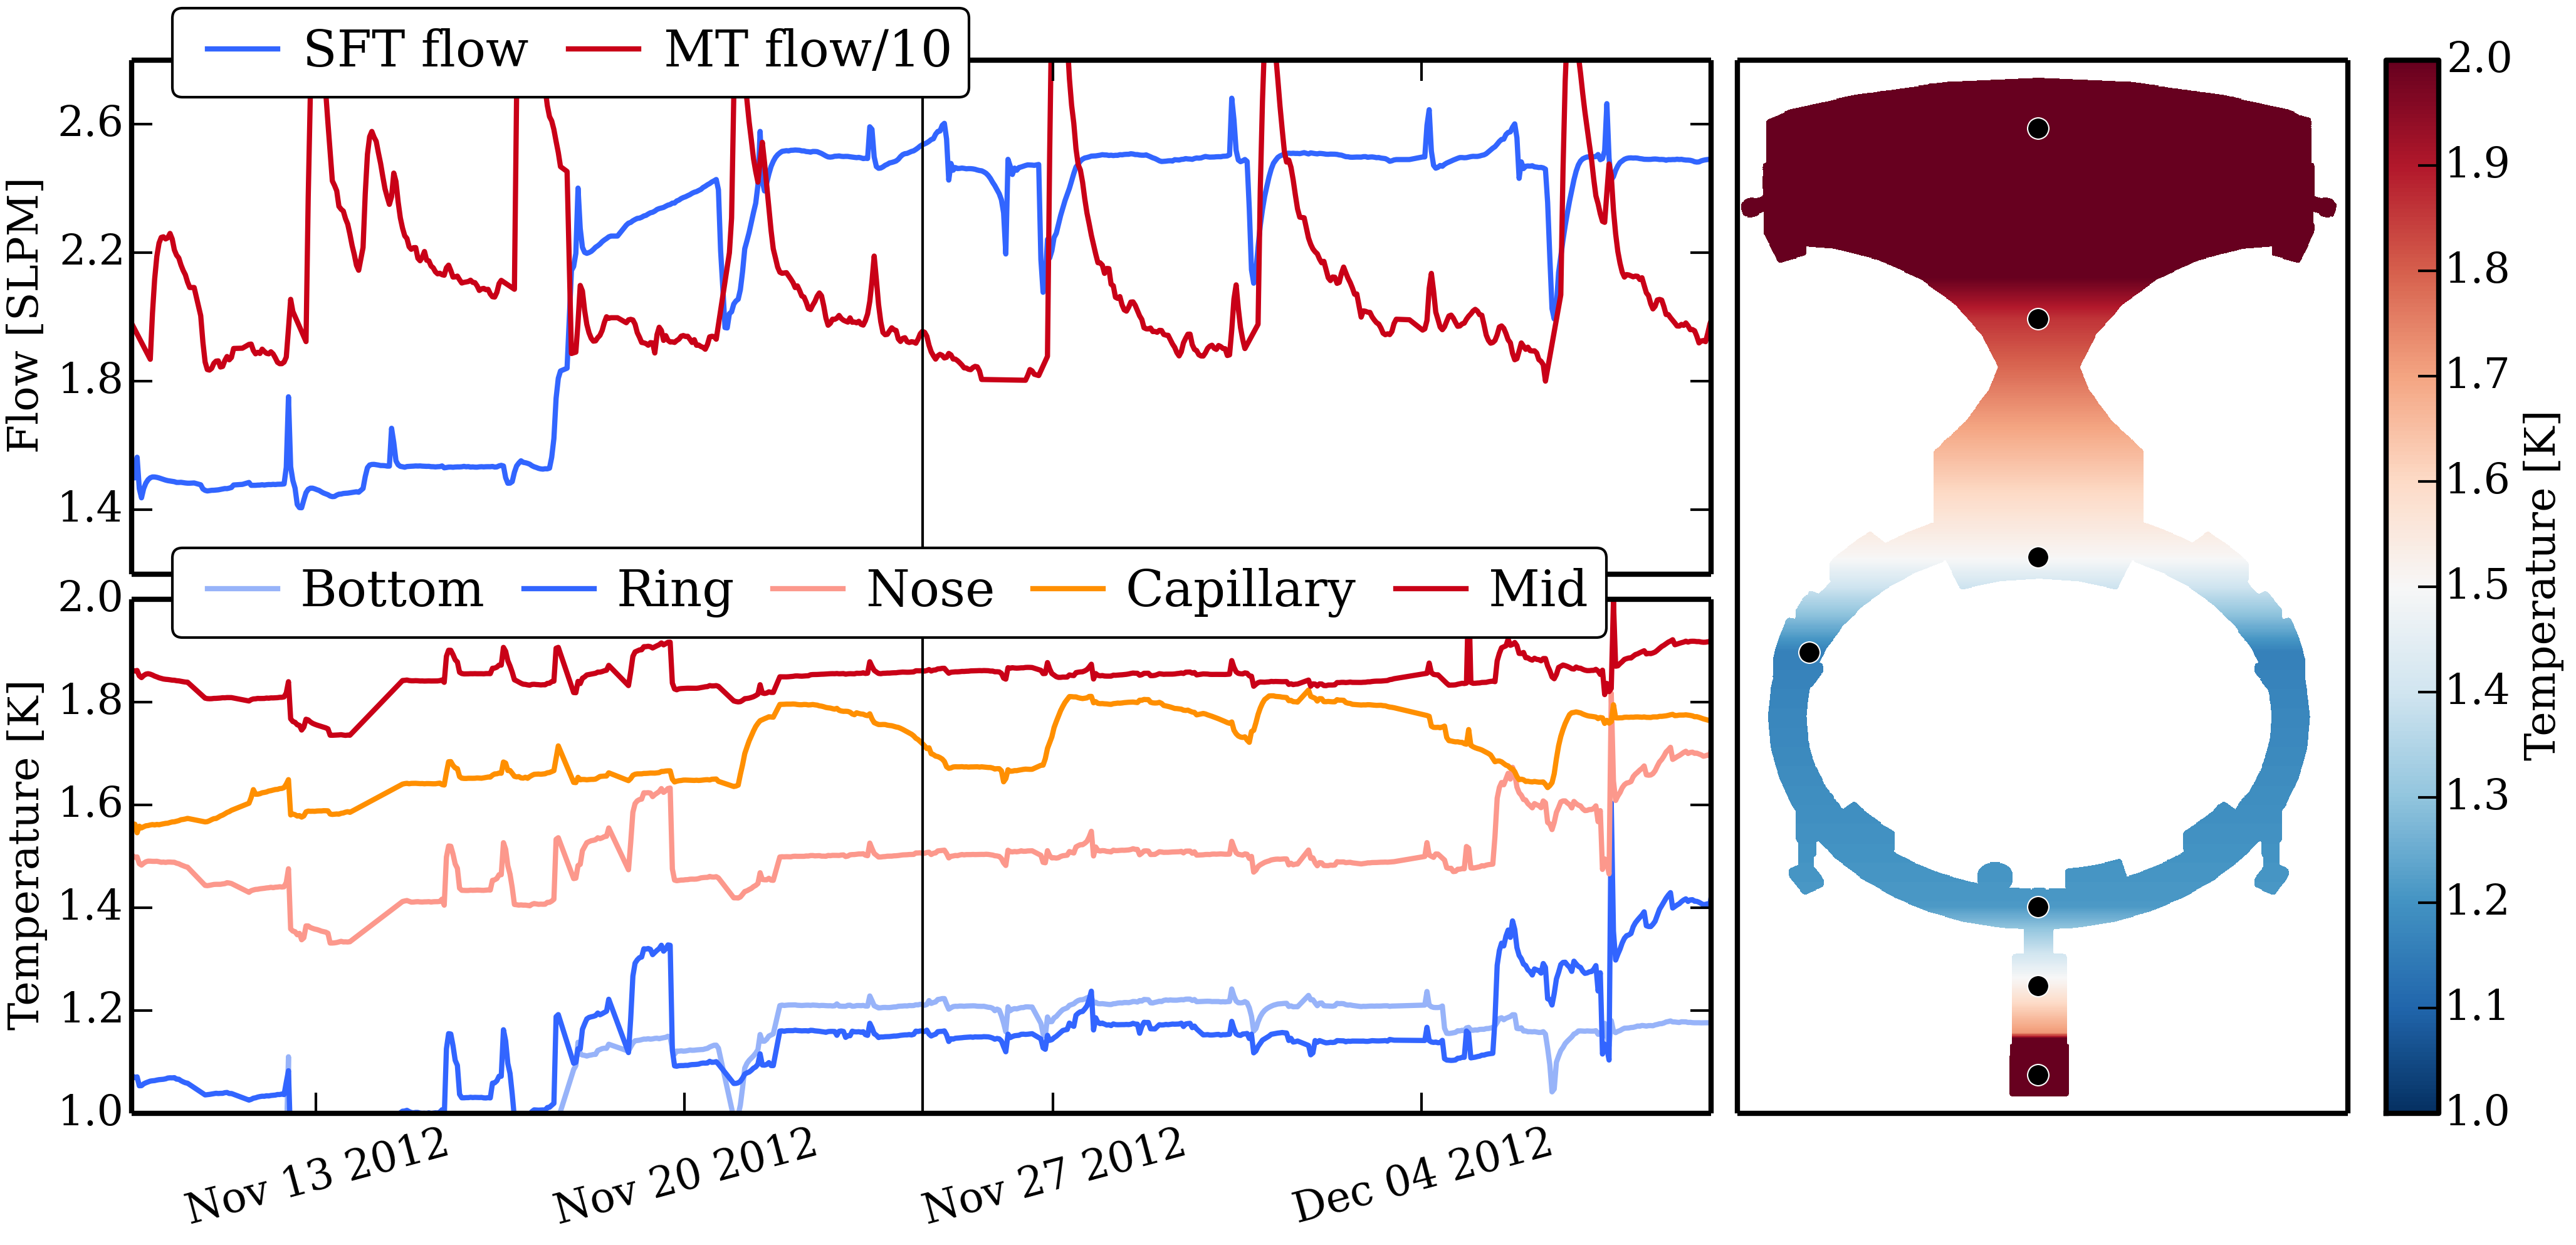
\includegraphics[width = 1.00\textwidth]{img/sft395.png}}
\end{center}
\caption[Cryogenic data from the MT and SFT]{\textit{Left above:} Flow rate out of the SFT and MT during a four week period during cryogenic testing in Princeton, Run 11. \textit{Left below:} Temperature of various parts of the SFT as a function of time for the same time period. \textit{Right:} A crude visualization of the temperature profile of the SFT at the time indicated by vertical line on the left-hand side plots. The black circles represent locations of thermometers.}
\label{fig:sft_hist}
\end{figure*} 

%\section{Conclusions}

%Insert text

%\section{Leak Checking}
%All parts were leak checked at some point in the assembly stage. These leak checks consisted of pulling a vacuum on the part and then spritzing the outside with helium while the part was at room temperature. No leaks were observed during these leak tests.

%\section{Capillaries}
%The following are notes on the capillaries that are currently installed in Wilbur. The number suggests how many have been made so far. Most capillary assemblies have failed when the capillaries are wound on the teflon spool or they have failed a flow test (no flow). The few capillary assemblies that in my mind went flawlessly did not pass the flow test. However, some of the more sketchy ones did.
%\begin{itemize}
%\item 2) One end pushed into tygon tube but that didn't work. Then cut and pushed through a helium stinger. Gas sent through while soldering. When doing the other end I forgot the female nut. Quickly realized this and so I heated it up again and slipped the nut on. Got slightly bent on one end.
%\item 5) Standard method. Maybe too little gas sent through during soldering of one end.
%\item 7) Standard method except that no He gas was sent through as one end was being soldered.
%\item 11) Standard soldering job on one end. For the other I forgot the female nut, AGAIN, and so I had to reflow the solder and slip it on.
%\end{itemize}
%All capillaries pass a flow test where we push a few psi of helium through and watch as bubbles form in water container. Unfortunately the flow is below the range of the flow meters that we have and so a quantitative estimate of the flow rates for each capillary has not been performed.

\bibliography{references}
\bibliographystyle{unsrt}

\end{document}
